\subsection{Know your user}
A large part of the objective outlined in section 3.1, design, is defined by the service that we want to offer
to the user. Asssisting the user, (our client), is our primary purpose. \\


We must be aware of the needs of users in order to meet their demands, as well as being aware of deficiencies in the market, so we can cover any 'holes'.
We should cater for all audiences equally 

Whether our target audience is unique, that is, take all types of users equally, considering the
average user, as for a characteristic user, we should know the homogeneous characteristics of our group.

Therefore we need a current study on the psychological, social and economic level of the target group, to ascertain not only
their needs, but also their wishes.

Once the users have access to the data we provide, it is important to have a feedback process.
It would be ideal to be able to perform an analysis of user behavior, to see their guidelines regarding the data obtained.
\subsubsection*{Suggested strategies} 
Define what type of user is intended. Study both their characteristics and the situation of the
market.
Use a mechanism that helps us obtain feedback, either by a system of points, test or
an automatic mechanism that allows tracking the behavior of the user. We can also choose the combination of both
options.

\subsubsection*{In the context of Aire Guru \ldots} 
Air Guru is aimed at the general population, therefore it's appropriate to present complete information in simple way. In addition, we pay special attention to users who may have a
disease or medical condition, caused or affected by, air pollution.
During the market study, we realized that many existing tools offered information about air pollution in real time, but we could see the following deficiencies:
\begin{itemize}
    \item Obsolete measurements. Measurements need to be taken regularly, since there can be huge differences
    between pollution levels at different times of the day.
    \item Limited geographic coverage. The data must cover a reasonable proportion of areas that people spend significant time in.
    \item Insufficiently granular measurements. Measurements must be at a reasonably fine level of granularity. One single measurement for an entire city is not useful.
    \item Poor presentation. Often the information is presented in an uninterpreted form, making it difficult for users to visualize, especially in a geographic sense.
    \item Poor discrimination and interpretation. Many tools show individual values as a number or a colour. This information is not
    enough for the user to take control of their exposure. Such visualizations are not really compelling. 
    \item Unnexistent costumized pollutan's exposure. We are interested to know to which levels of pullutions we are exposed on the long term, no only in a determinate time.
    \item Need to use complicated devices to monitor the exposition. Our gol is to facilitate the information to the user with the minimal complication for them.
    \item No related information about pollutans and their influence on our health or medical conditions.
\end{itemize}

Once implemented, we tested the tool with 14 users. Our tool integrates Google Analytics that allow us to evaluate
user behavior, how many pages they access, and how long they stay on them. Also, after the test, we conducted a survey to measure not only the level of satisfaction with the tool, but also to verify the utility and if the user was able to achieve their objective.
\begin{figure}[ht]
    \centering
   \subfigure[Aire Guru Form]
    {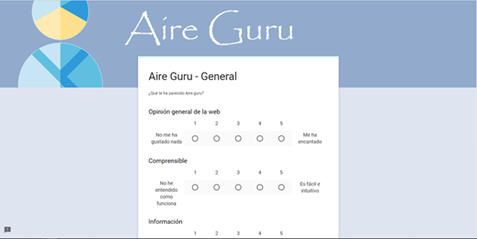
\includegraphics[width=5.5cm  ]{form}}
    \hfill
    \subfigure [Google Analytics]
       { 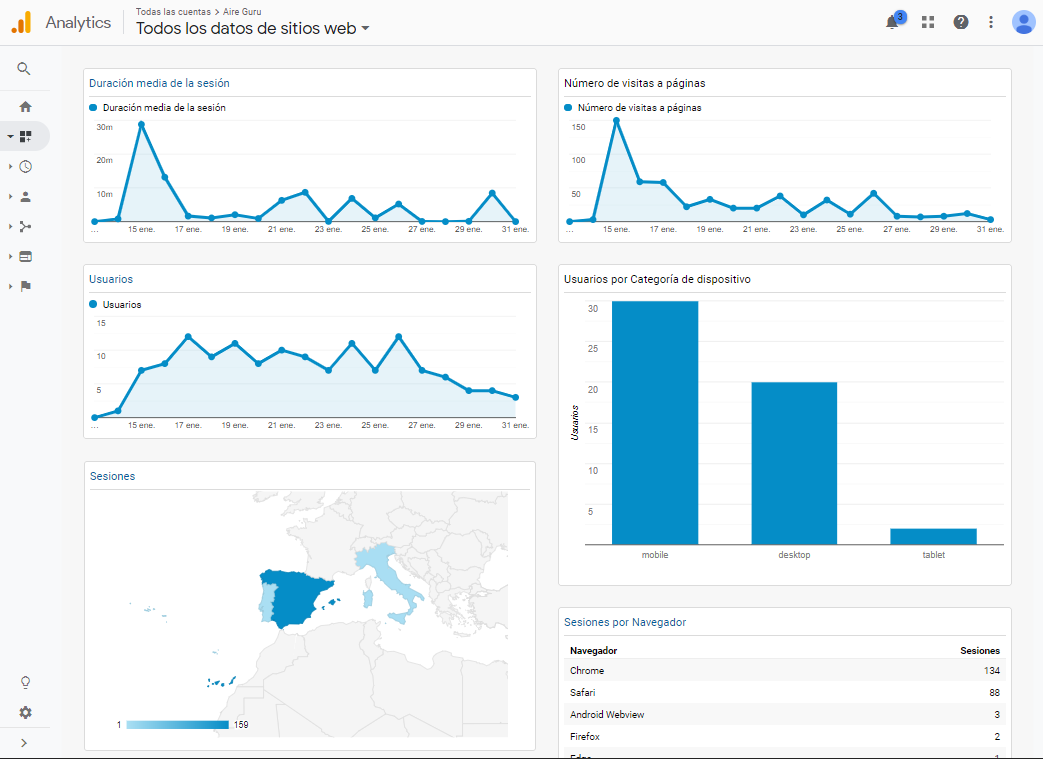
\includegraphics[width=5.5cm]{googleAnalytics}}
  
  \caption{User Feedback}
    \end{figure}
 
\elsparagraph{Evaluation}  
\begin{itemize}
    \done The market study made us clearly see the shortcomings that exist in current applications.
    \done The survey gave us positive evaluations regarding the useability, interpretability, and depth of information reported.
    \done Thanks to Aire Guru, users noticed about medical conditions with the potential to affect them personally, that could be caused or made worse by air pollution.

\end{itemize}